%!TEX root = dissertation.tex
%%%%%%%%%%%%%%%%%%%%%%%%%%%%%%%%%%%%%%%%%%%%%%%%%%%%%%%%%%%%%%%%%%%%%%%%%%%%%%%%
\chapter{Streaming in Mobile Networks}



%%%%%%%%%%%%%%%%%%%%%%%%%%%%%%%%%%%%%%%%%%%%%%%%%%%%%%%%%%%%%%%%%%%%%%%%%%%%%%%%
\section{Streaming Mobile Adaptation}



%%%%%%%%%%%%%%%%%%%%%%%%%%%%%%%%%%%%%%%%%%%%%%%%%%%%%%%%%%%%%%%%%%%%%%%%%%%%%%%%
\section{Influences of Layers}
\subsection{Peculiarities of the Transport Plane}
\subsection{The Question of Network Support}




Wired Internet access has a very narrow choice of protocols on the ISO/OSI Layers 1 and 2. The typical use-case consists of a Local Area Network using Ethernet which is then tunneled through or translated into one of several access technologies, e.g., DSL, DOCSIS, or PON. Applications often make assumptions that rely on the presence of these protocols and their specific characteristics.

However, Internet access today is similarly often achieved using mobile cellular networks. The latest standardized iteration of these is LTE and the accompanying EPS core network infrastructure \cite{olsson2009sae}. This is the first evolution of standards that completely removes the classical circuit switched domain making room for more radio frequency bandwidth to be used with the all-IP services achieving shared transmission capacities -- comparable to today's 802.11n WiFi -- albeit on much larger cell sizes of 1 to 30 kilometres. The EPS network (cf. Fig. fig:ltecore) acts as an intermediary between the radio access stations and the Internet enabling strong traffic control mechanisms as well as mobility anchored at the Serving Gateway (S-GW). Traffic is routed through the core by using tunneling over the S-GW and P-GW based on the traffic bearer concept defined either in the GTP or the PMIPv6 protocols. For every mobile device connected to the network there is one default and up to ten dedicated bearers carrying traffic filtered by pre-set QoS parameters. Control is enforced through a logically separate network control plane, that is also used to setup and tear down these bearers. Figure fig:ltestack displays the disparity between the Internet's protocol stack and that of an LTE network encapsulating all user traffic in additional protocol layers by the tunneling process.

Research work is ongoing how to best work with this complex network setup. It is expected, that with the rise of mobile access the core network comes under heavy traffic pressure with negative affects on the QoS of best-effort traffic. Endeavors are required to study the loaded network's behavior. Also very little work has gone into exploring the control plane characteristics of these networks, including their performance. A novel approach could also be, to make mobile device applications, e.g. video streaming players, aware of the core networks capabilities and allow the request of tunnels tailored to their specific QoS requirements resulting in a possible increase of perceived quality.

% influence of signaling plane and core network elements - scaling

The protocols used for the radio transmissions behave very differently when compared to Ethernet and assumptions made by higher layers may not hold any more. This can apply to, e.g., reliability, frame sizing and fragmenting, and latency amounting to undesired effects on higher-layer traffic. For example, loss in GSM and UMTS networks is often caught transparently on layer 2 and a retransmission is conducted. However, in the time the retransmission takes the transport layer may have already run into a timeout and re-requested the missing segment on its own, resulting in additional delay and a waste of bandwidth. This is especially detrimental for time-critical applications like video streaming, possibly resulting in buffer underruns and degraded quality. Transport and application layer mechanisms need to be able to understand this and cope with the effects. E.g., TCP retransmissions and congestion control could be adjusted in the course of understanding this.

Furthermore, traffic could be avoided during cell handover occurrences. This would require cross-layer cooperation and an awareness of the application when an handover is supposed to occur. The application then could schedule its traffic accordingly. Traffic falling into a handover is subject to especially high latency and loss because the mobile network acts as a mobility anchor which needs to internally reroute incoming traffic to the mobile device's new position. HTTP traffic is especially suited to this scheduling behavior because of its statelessness and consistence of small objects that can be requested and transferred independently.


\begin{figure}
\centering

%\subfloat[LTE tunneling concepts.]{\label{fig:ltetunneling}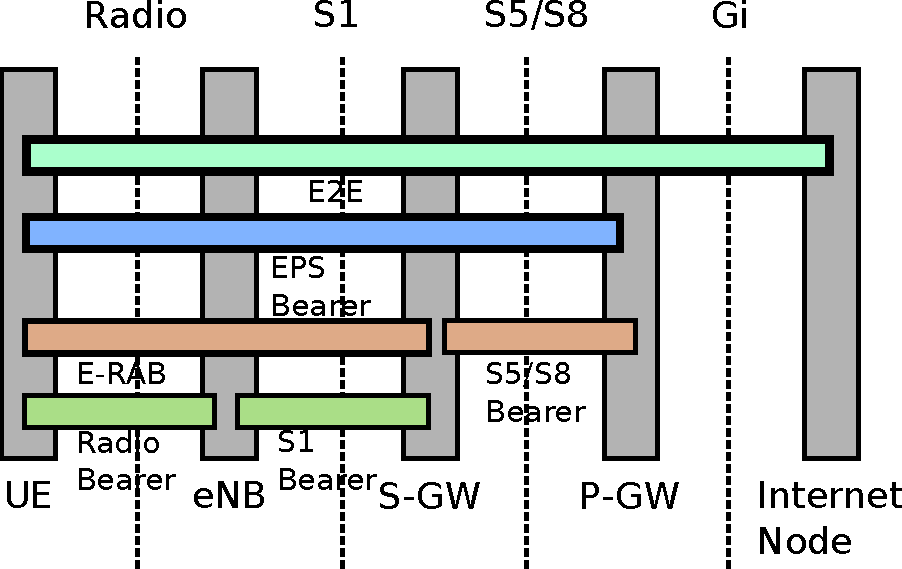
\includegraphics[width=0.4\textwidth]{ltetunneling.pdf}}
%\hfil
%\subfloat[Minimal working subset of a LTE and EPS architecture.]{\label{fig:ltecore}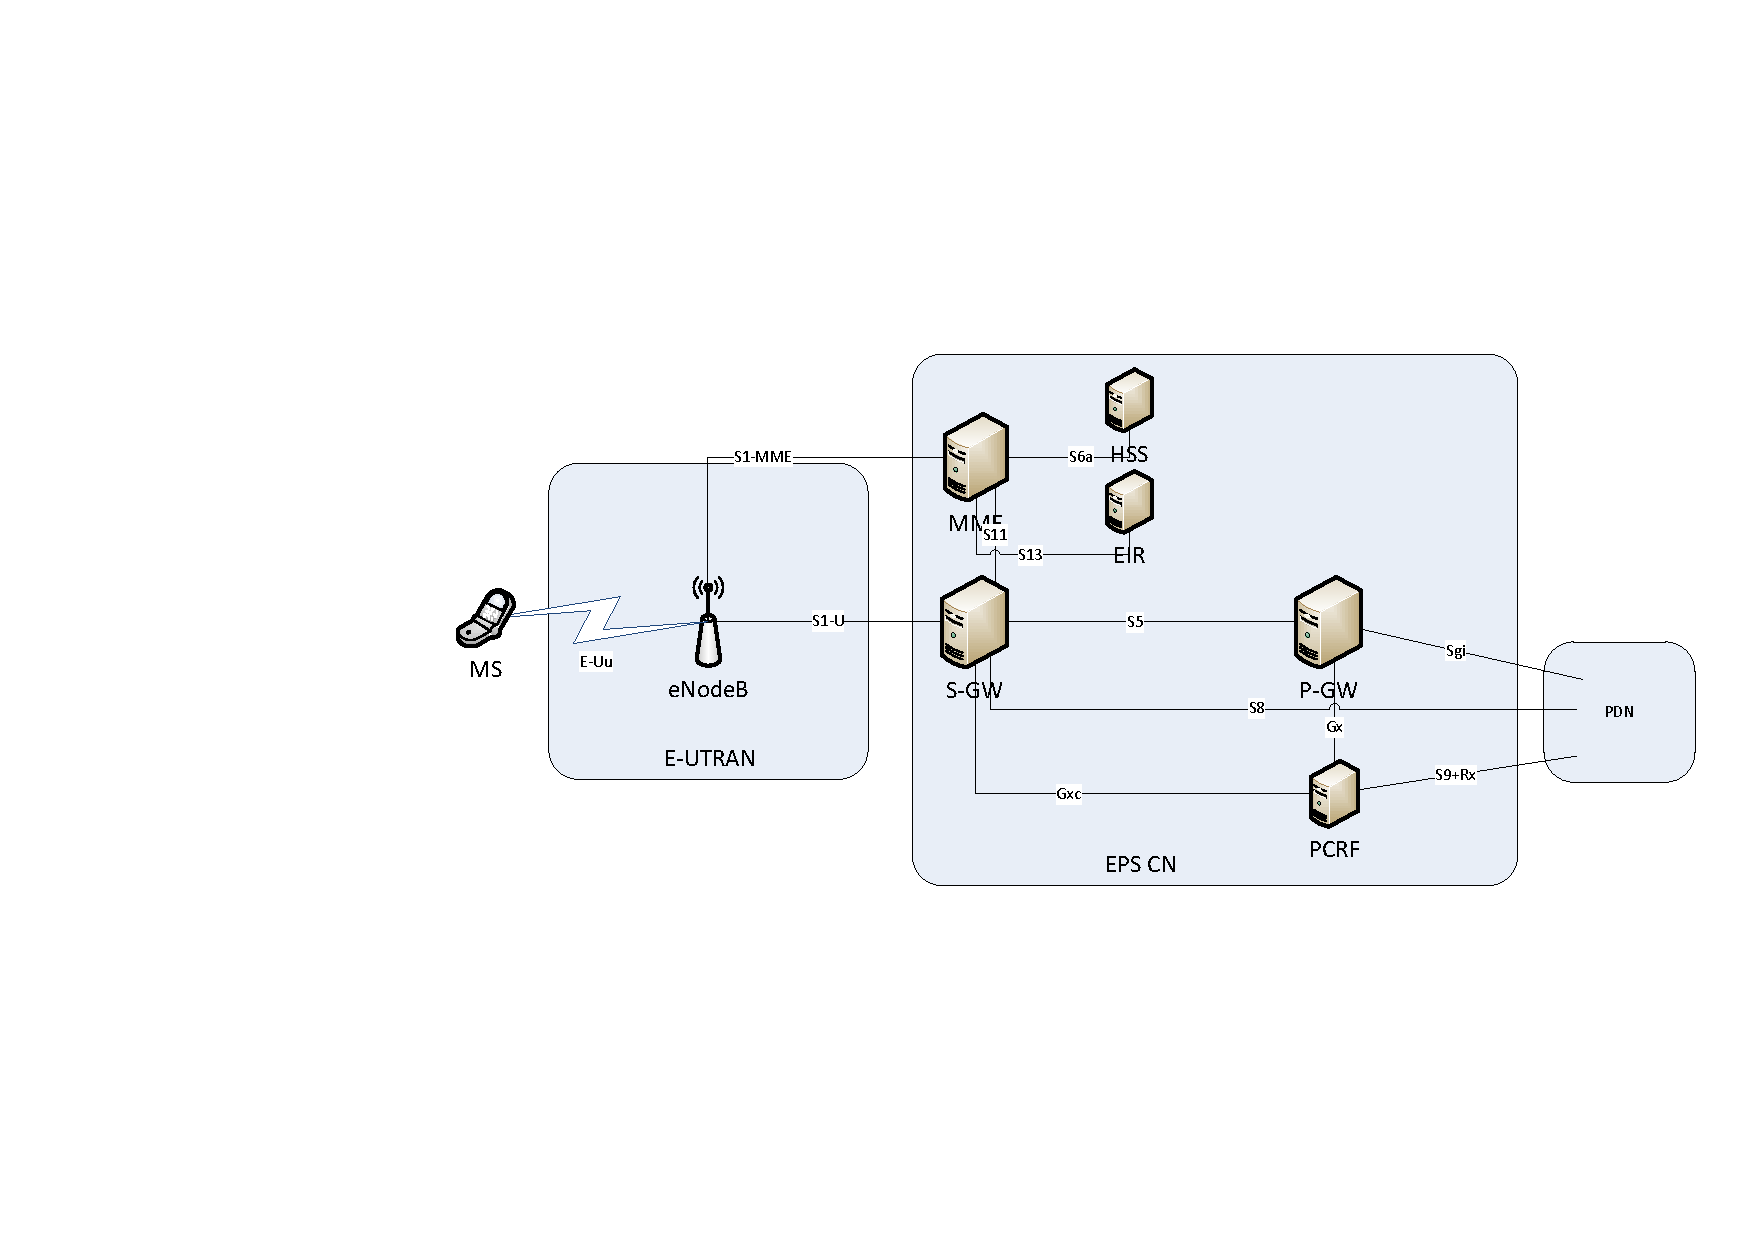
\includegraphics[width=0.6\textwidth]{lte-core.pdf}}\\

%\subfloat[LTE protocol stack.]{\label{fig:ltestack}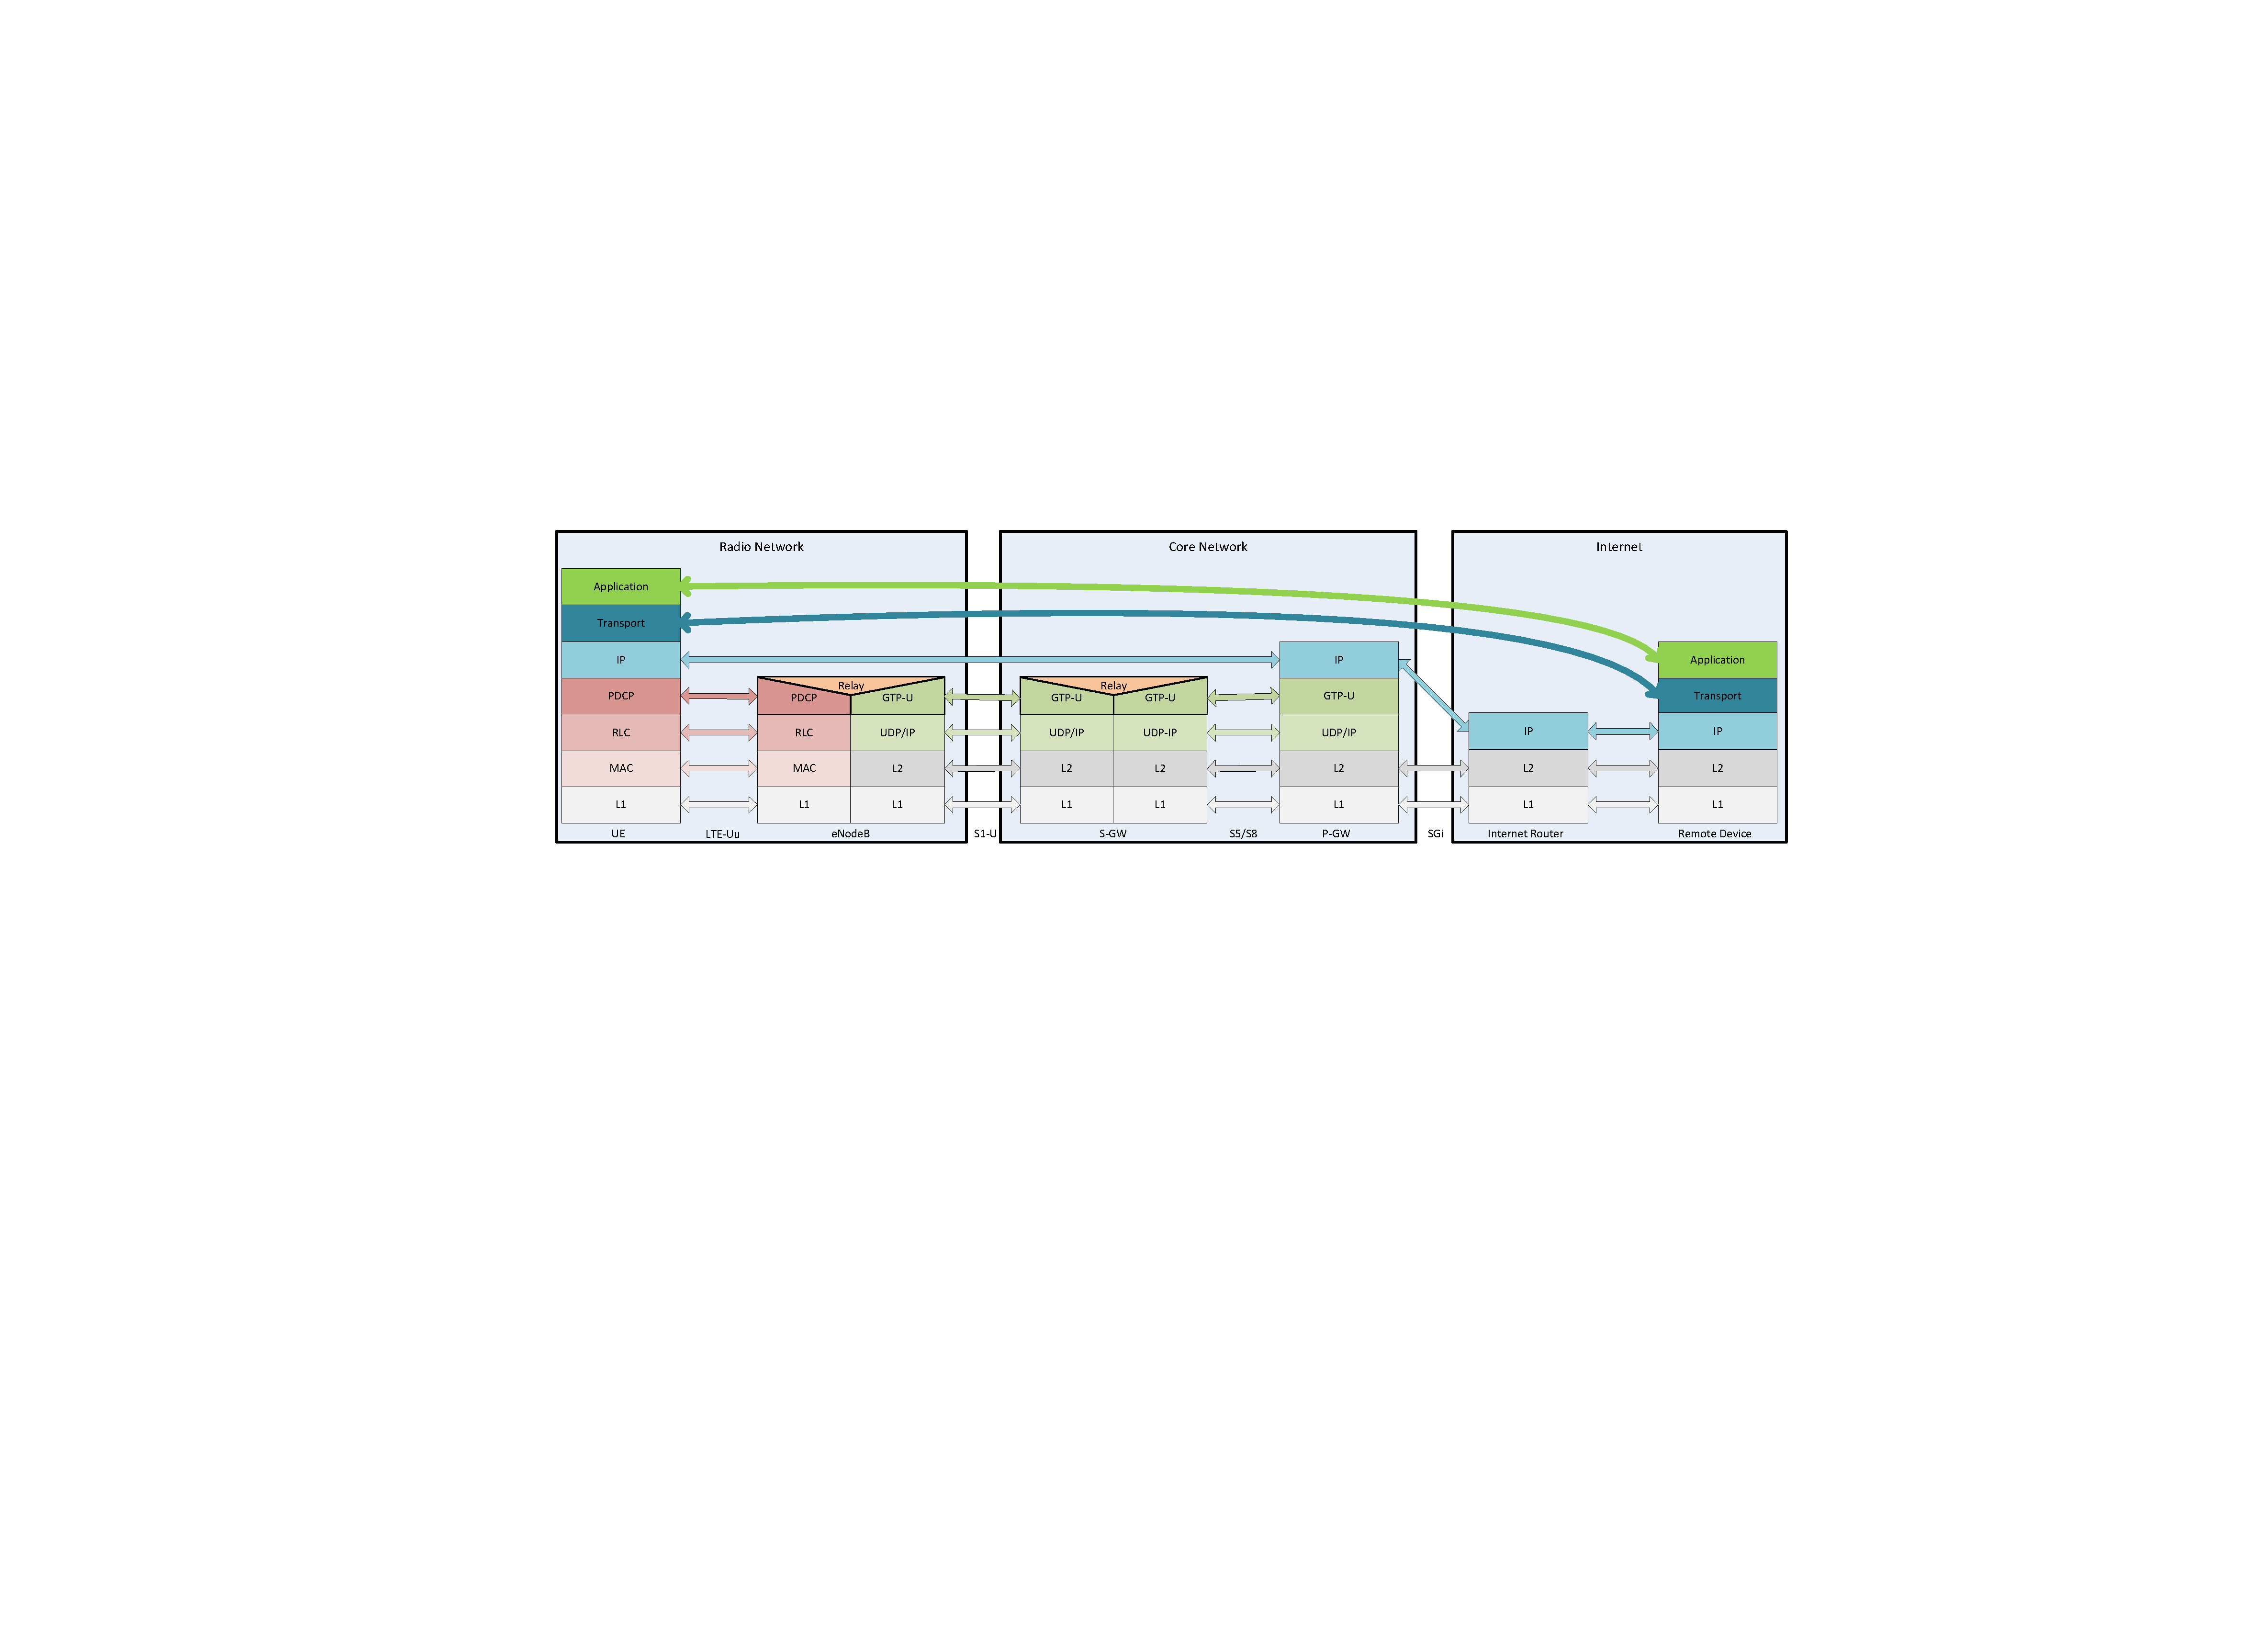
\includegraphics[width=1.0\textwidth]{ltestack.pdf}}
\caption{LTE concepts and architecture.}
\label{fig:lte}
\end{figure}





%%%%%%%%%%%%%%%%%%%%%%%%%%%%%%%%%%%%%%%%%%%%%%%%%%%%%%%%%%%%%%%%%%%%%%%%%%%%%%%%
\section{System Analysis}
\subsection{Mobile Streaming Simulation/Emulation Hybrid Test Platform}

Use introduced streaming evaluation approaches in a mobile network environment

But do not want to use real network, as conditions are hard to manage and reproduce. Additionally, LTE still hard to come by.

Therefore, use an emulated network provided by the ns-3 network simulator. But transmit real traffic through it, i.e. use it as an emulator and bridges. \ref{fig:lte-testbed}

\begin{figure}
\centering
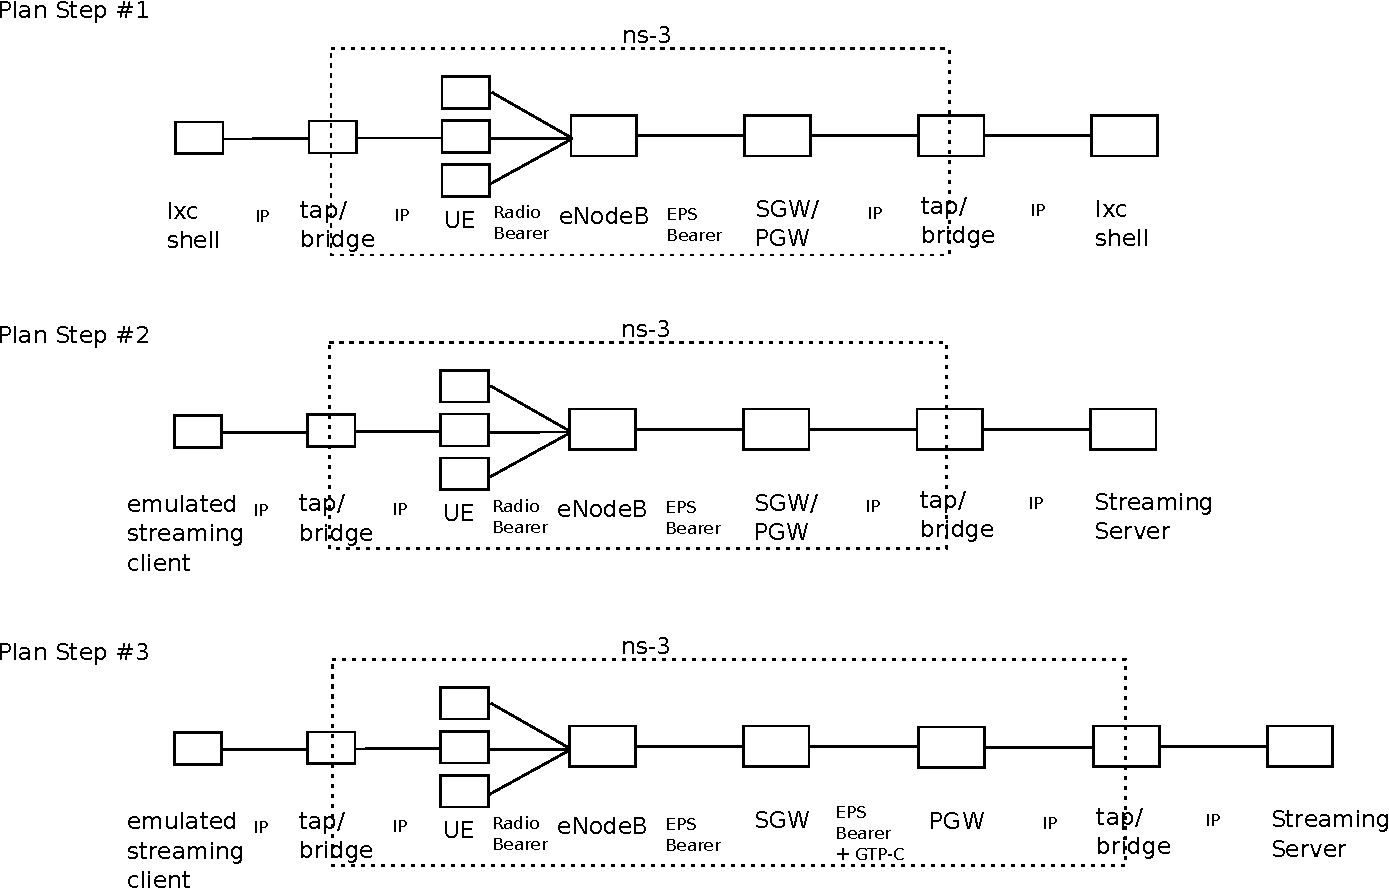
\includegraphics[width=\textwidth]{images/lte-testbed.pdf}
\caption{LTE Streaming Evaluation Setup and Action Plan}
\label{fig:lte-testbed}
\end{figure}